\section{Block Modes}
\subsection{Electronic Codebook - ECB}
\begin{wrapfigure}{r}{0.3\textwidth}
\vspace{-20pt}
\fbox{
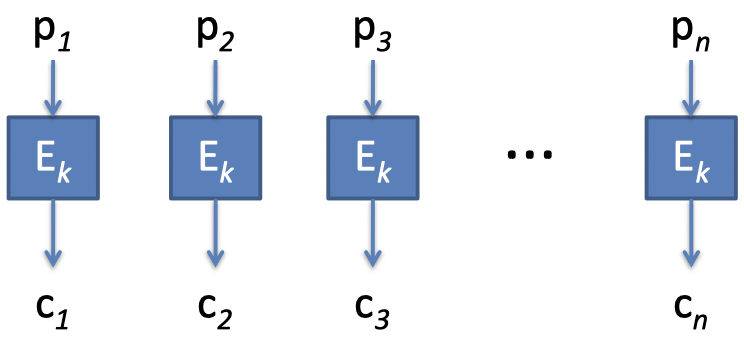
\includegraphics[scale=0.5]{images/ecb.png}}
\end{wrapfigure}
Simplest block mode, just cut the message into $m-$bit blocks and apply the cipher function to each block. 
The problem is that if we repeat a plaintext block, we obtain the same cipher blocks. A first way to improve ECB would be to XOR each plaintext block with random number, but still we will have problems: now we have twice as much data to transmit and message modification is easy.

\subsection{Cipher Block Chaining - CBC}
\begin{wrapfigure}{r}{0.3\textwidth}
\vspace{-50pt}
\fbox{
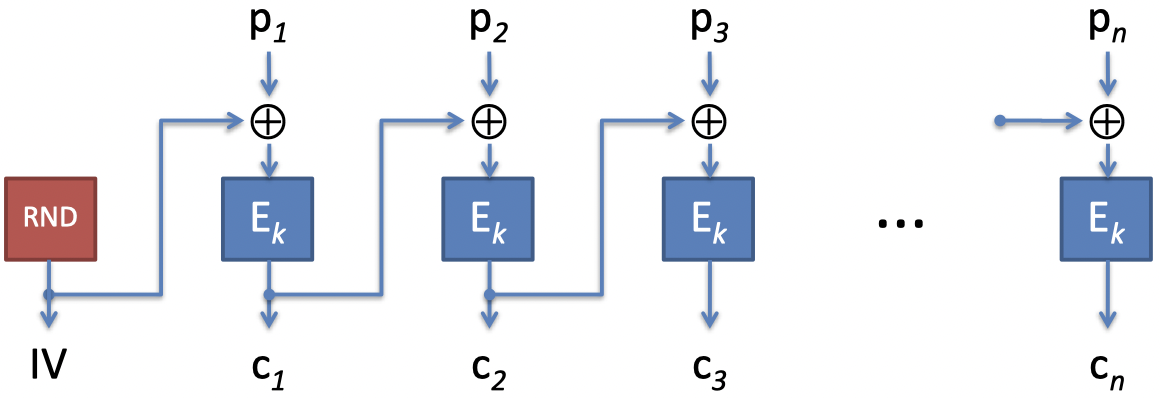
\includegraphics[scale=0.35]{images/cbc.png}}
\end{wrapfigure}
Each block of plaintext is XORed with the preceeding block of ciphertext before encryption. It uses a random \textit{initialisation vector} $IV$ that should never be reused and should stay secret.


\subsection{Cipher Feedback - CFB}
\begin{wrapfigure}{r}{0.3\textwidth}
\vspace{-60pt}
\fbox{
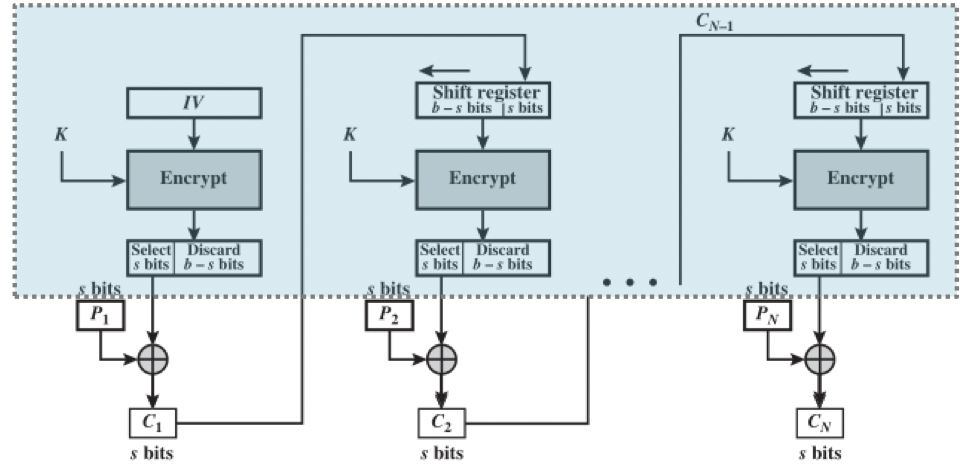
\includegraphics[scale=0.4]{images/cfb.png}}
\end{wrapfigure}
Preceeding ciphertext is used as input to encryption algorithm, to produce pseudorandom output that is XORed with plaintext. Can work on subset of $j$ bits instead of entire blocks.


\subsection{Counter Mode - CTR}
\begin{wrapfigure}{r}{0.3\textwidth}
\vspace{-50pt}
\fbox{
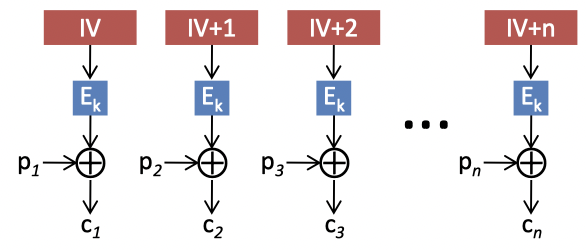
\includegraphics[scale=0.55]{images/ctr.png}}
\end{wrapfigure}
Each plaintext block is XORed to encrypted counter. Counter gets incremented for each subsequent block.


\begin{wrapfigure}{r}{0.3\textwidth}
\vspace{-50pt}
\fbox{
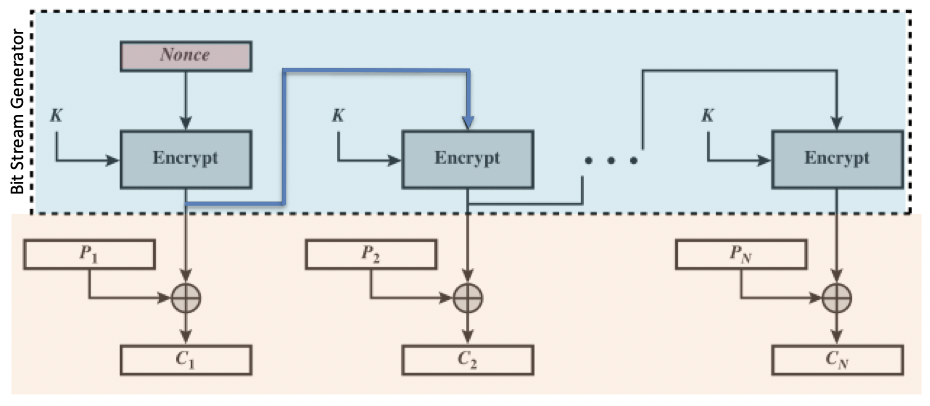
\includegraphics[scale=0.4]{images/ofb.png}}
\end{wrapfigure}
\subsection{Output Feedback - OFB}
Similar to CFB, except that instead of ciphertext, it uses preceeding output of encryption function as input to the successive encryption function.
